%!TEX root = ../thesis-summary.tex

\section{Implementation}
\label{section:implementation}

For our Pulsarcast implementation, we decided to take advantage of the
\emph{libp2p} ecosystem as it solves a lot of the underlying issues of building
a peer to peer system, not specific to our pub-sub scenario. This includes
dealing with connection multiplexing, NAT traversal, discovery mechanisms and
others. We can also take advantage of the utility modules it has and the
advantage of having an already working implementation of the Kadmelia DHT. Our
focus is then to build a module, implementing the Pulsarcast specification that
clients and apps can take advantage of. 

We chose to implement our Pulsarcast module in Javascript. As we covered in our
related work, Javascript is ubiquitous, running in browsers, servers and many
different kinds of devices and architectures. Through it, we can run our
Pulscarcast nodes in a multitude of systems and most importantly, direct its
usage for the World Wide Web. Plus, libp2p has a Javascript implementation
focused on cross-compatibility between server and browser. It is worth
noting that, much like the work we built on top of, this module is open
source~\footnote{\url{https://github.com/JGAntunes/js-pulsarcast}}.

Figure \ref{fig:pulsarcast-in-libp2p} gives us an overview of how our module
fits in the libp2p ecosystem. libp2p defines interfaces responsible for routing
content (peer routing), discovering other peers in the network (peer
discovery), network transports and leveraging multiple network connections
(switch). These all come bundled in the libp2p javascript
module~\footnote{\url{https://github.com/libp2p/js-libp2}} which we use in
Pulsarcast. Besides the main libp2p module we also use some other utility
modules such as the CID
module~\footnote{\url{https://github.com/multiformats/js-cid}} and the Peer-id
module~\footnote{\url{https://github.com/libp2p/js-peer-id}}, both designed to
reason with content identifiers (peer identifiers are also content
identifiers). 

\begin{figure}[hb!]
  \centering
  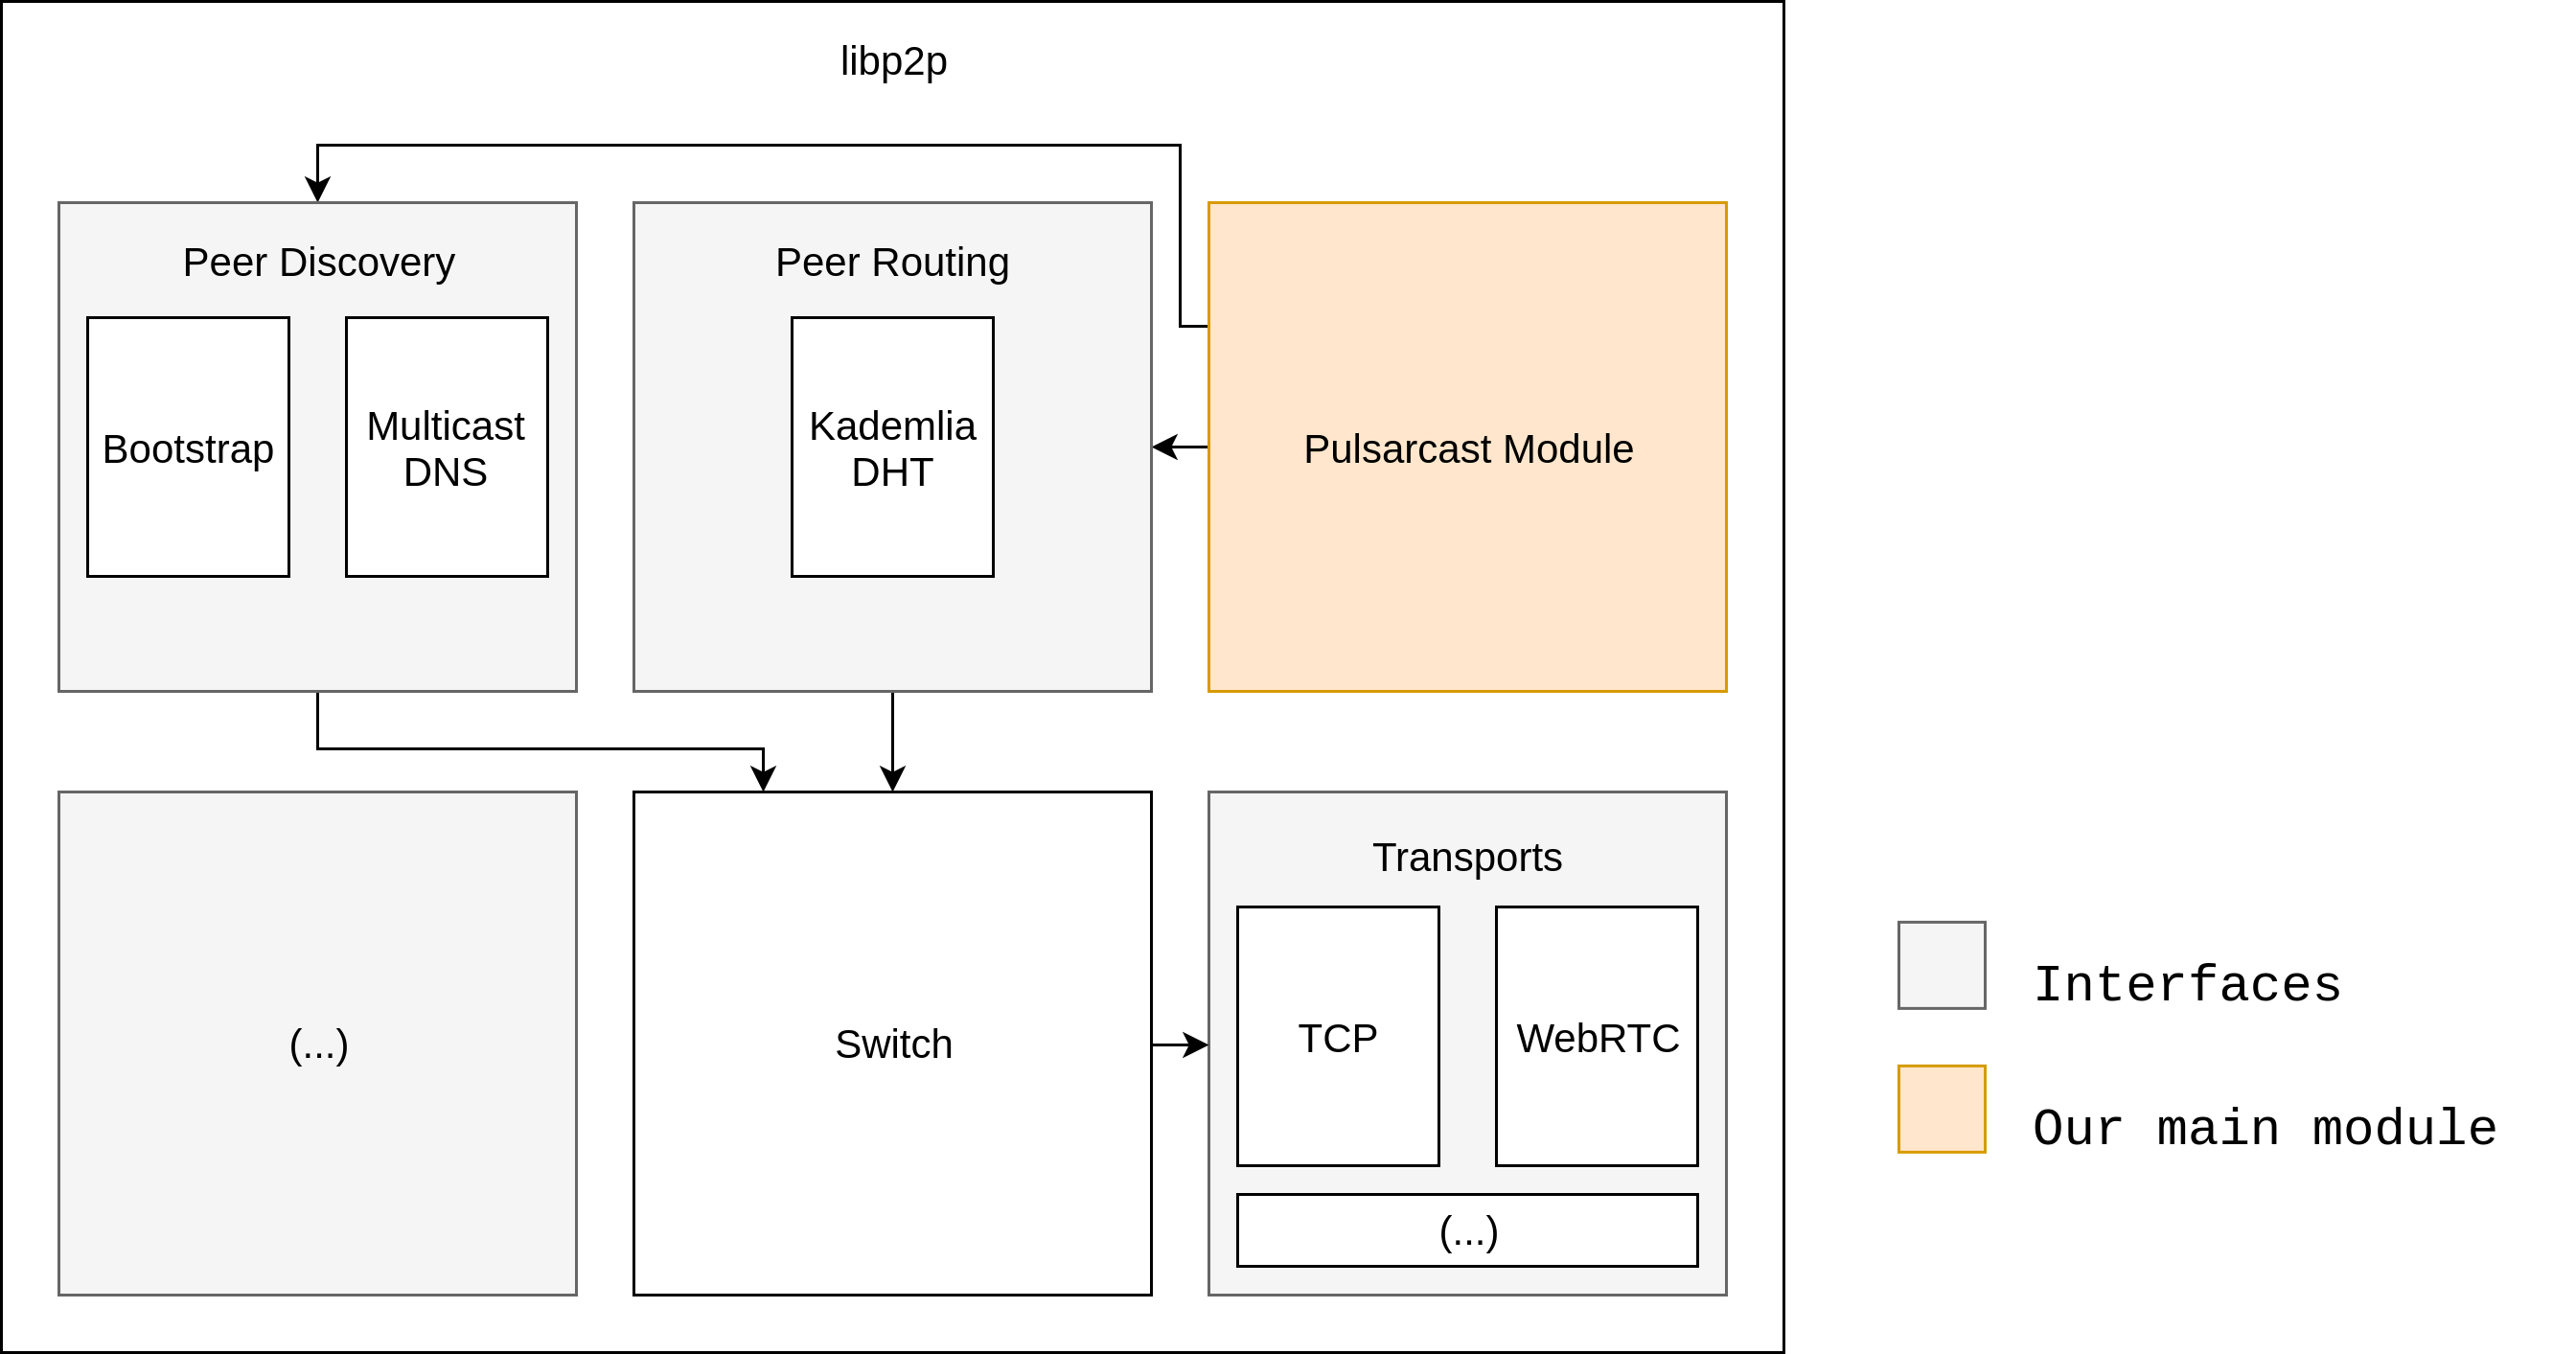
\includegraphics[width=0.4\textwidth]{img/pulsarcast-in-libp2p.png}
  \caption{Our Pulsarcast module in the libp2p ecosystem}
  \label{fig:pulsarcast-in-libp2p}
\end{figure}


Pulsarcast has five classes. These are:

\begin{itemize}
  \item
    Pulsarcast - Our main class, responsible for holding the state of our node, managing peer lists and connections. It extends the built-in \verb|EventEmitter| class~\footnote{\url{https://nodejs.org/api/events.html}}, making our class capable of reproducing the event emitter pattern~\footnote{\url{https://nodejs.dev/the-nodejs-event-emitter}}, the mechanism we use to bubble up new Pulsarcast events to the application level.
  \item
		Peer - An abstraction for the state of each peer, including connections, identifiers, adresses and dissemination trees.
  \item
    TopicNode - Abstracts the Topic descriptor for our Merkle DAG.
  \item
    EventNode - Just as above, abstracts the Event descriptor for our Merkle DAG.
  \item
    EventTree - Manages the state of the event tree for each topic.
\end{itemize}

Listing \ref{pulsarcast-usage-example} provides a usage example of our
Javascript module. Keep in mind that this is a oversimplified example of
course, with a single node, its purpose is to understand how the
API~\footnote{The full documented API for our module - \url{https://github.com/JGAntunes/js-pulsarcast/blob/547ff33527f0df8c751d5fcd73d559fce59cdb77/docs/api.md}}
comes together and allows applications to integrate with it.

\begin{lstlisting}[language=JavaScript, float=h, caption={Usage example of our Pulsarcast module},label={pulsarcast-usage-example}]
const Pulsarcast = require('pulsarcast')

// node is a libp2p Node
const pulsarcastNode = new Pulsarcast(node)

const pulsarcastNode.start((err) => {
  if (err) console.log('No!!!', err)
  
  pulsarcastNode.createTopic('fuuuuun', (err, cid, topicNode) => {
    if (err) console.log('No!!!', err)
    console.log('Our new topic \o/', topicNode)
    
    pulsarcastNode.on(cid.toBaseEncodedString(), (eventNode) => {
      console.log('event', eventNode)
    })
    
    pulsarcastNode.publish(cid.toBaseEncodedString(), new Buffer('super fun!'), (err, eventCID) => {
      if (err) console.log('No!!!', err)
      console.log('published', eventCID.toBaseEncodedString())
    })
  })
})
\end{lstlisting}

